\chapter{Réduction des endomorphismes}
On écrivant ce chapitre, j'étais inspiré par les videos du chaîne \textit{3blue1brown} que je vous conseille regarder, au moins le playlist concernant l'algèbre linéaire. La deuxieme source de l'inspiration était le livre de Joseph Grifone \cite{grifone}.
\section{Introduction}
Dans le chapitre précédent on a étudier une notion d'une base orthonormale dont les utilités sont: simplification des calcule des coordonnées dans une base et calcule d'une projection. 
Cette notion est l'un des premiers pas vers l'étude de SVD\footnote{Singular Value Decomposition} qui est appliqué dans plusieurs domaines, e.g: la réduction des tailles d'images.
\par
Dans ce chapitre on continue l'étude des bases pour pouvoir finalement comprendre le SVD. On va étudier la réduction des endomorphismes, \textit{to be more precise} la diagonalisation et la triagonalisation. Pour commencer: un petit exo:
\begin{ex}
   Calculer 
   \[
   \begin{bmatrix} 
       3 & 1\\
       0 & 2
   \end{bmatrix}^{15} = \underbrace{
       \begin{bmatrix} 
       3 & 1\\
       0 & 2
       \end{bmatrix}
       \cdot
       \ldots
       \cdot
       \begin{bmatrix} 
       3 & 1\\
       0 & 2
       \end{bmatrix}
   }_{15 \text{ fois}}
   \] 
\end{ex}
Cela ne semble pas très facile, n'est-ce pas? Au bout de ce chapitre, on va trouver une façon à simplifier le calcule et à la fin on résoudra cet exercice.
\par
On sait d'algèbre linéaire qu'on peut représenter une matrice d'une application dans des bases différentes, i.e soit une base $\{e_i\}$ de $E$ et  $f$ une application. Alors cette aplication dans la base  $\{e_i\}$ est représentée:
 \[
A = M(f)_{e_i} = \|f(e_1), \ldots, f(e_n)\|
\] 
Soit $\{e_i'\}$ une autre base de  $E$, alors on peut représenter l'application  $f$ dans cette base aussi, notons:  $P = P_{e_i \to e_i'}$ une matrice de passage de la base $\{e_i\}$ vers la base  $\{e_i'\}$
 \[
     A' = M(f)_{e_i'} = P^{-1}AP = \|f(e_1'), \ldots, f(e_n')\|_{e_i'}
\] 
\begin{definition}\label{def:matrice-diagonalisable}
    La matrice $A$ est \textbf{diagonalisable} s'il existe une matrice semblable  $A'$ diagonale:
     \[
         A' = 
         \begin{bmatrix} 
         a_{1,1} & 0 & \ldots & 0 \\
         0 & a_{2,2} & \ddots & \vdots\\
         \vdots & \ddots & \ddots & 0\\
         0 & \ldots & 0 & a_{n,n}
        \end{bmatrix} 
    \] 
\end{definition}
\begin{definition}
    La matrice $A$ est \textbf{triagonalisable} s'il existe une matrice semblable  $A'$ triangulaire (supérieure/inférieure) 
     \[
         A' = 
         \begin{bmatrix} 
         a_{1,1} & a_{1,2} & \ldots & a_{1,n} \\
         0 & a_{2,2} & \ddots & \vdots\\
         \vdots & \ddots & \ddots & a_{n-1,n}\\
         0 & \ldots & 0 & a_{n,n}
        \end{bmatrix} \text{ ou } 
         A' = 
         \begin{bmatrix} 
         a_{1,1} & 0 & \ldots & 0 \\
         a_{2, 1} & a_{2,2} & \ddots & \vdots\\
         \vdots & \ddots & \ddots & 0\\
         a_{n, 1} & \ldots & a_{n, n-1} & a_{n,n}
        \end{bmatrix} 
    \] 
\end{definition}
Alors les problèmes de ce chapitre qu'on va résoudre sont:
\begin{enumerate}
    \item Détérminer si un endomorphisme $f$ est diagonalisable/triagonalisable i.e s'il existe telle matrice  $A'$.
    \item Détérminer la matrice de passage $P$ et la matrice $A'$.
\end{enumerate}
Dans tout le chapitre on suppose que l'espace vectoriel $E$ est de dimension finie.
\section{Vecteurs propres - Eigenvectors}
Commençons par clarification d'une notion de l'application linéaire et sa matrice. Preonons pour ça la matrice de l'exercice du début du chapitre:
\[
A = \begin{bmatrix} 
       3 & 1\\
       0 & 2
   \end{bmatrix}
\] 
Cetter matrice transforme l'espace vectoriel qu'on le donne, ou en simplifiant, elle transforme chaque vecteur de l'espace vectoriel. Prennons un vecteur $v_3 = \begin{pmatrix} 1 \\ 1 \end{pmatrix} $, en appliquant $A$ on obtient:
 \[
Av_3 = \begin{bmatrix} 
       3 & 1\\
       0 & 2
   \end{bmatrix}\begin{bmatrix} 1 \\ 1 \end{bmatrix} = \begin{bmatrix} 3 \\ 0 \end{bmatrix} + \begin{pmatrix} 1 \\ 2 \end{pmatrix} = \begin{bmatrix} 4 \\ 2 \end{bmatrix} 
\] 

\begin{center}
    
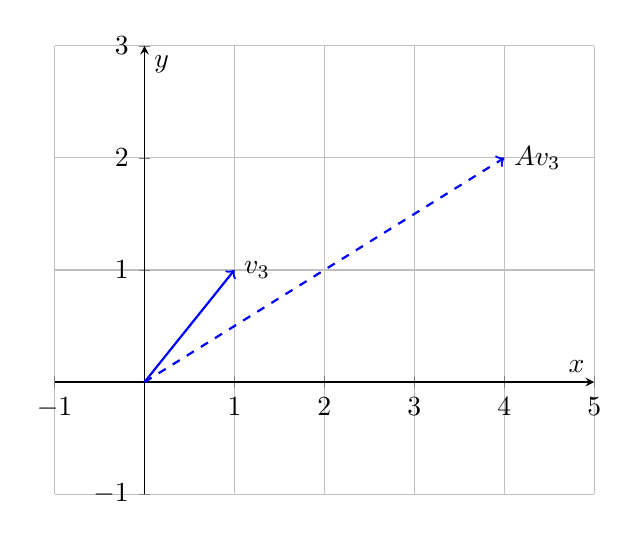
\begin{tikzpicture}
    \begin{axis}[
        axis lines=middle, 
        grid=major, 
        xlabel={$x$}, 
        ylabel={$y$}, 
        ymin=-1, ymax=3,
        xmin=-1, xmax=5
    ]
        % Define original vectors
        \addplot[->, thick, blue] coordinates {(0,0) (1,1)};
        \node[right] at (axis cs:1,1) {$v_3$};

        % Define transformed vectors
        \addplot[->, thick, blue, dashed] coordinates {(0,0) (4,2)};
        \node[right] at (axis cs:4,2) {$A v_3$};
    \end{axis}
\end{tikzpicture}
\end{center}
On remarque que le vecteur $Av_3$ n'est plus situé en même ligne que le vecteur $v_3$, ce qui est logique car si les vecteurs étaient en même lignes après une transformation, cela n'aurait pas de sens.
Par contre, parfois il y'a des cas, quand le vecteur appliqué à la matrice reste en même ligne, par exemple le vecteur $v_2 = \begin{pmatrix} -1 \\ 1 \end{pmatrix} $, avec $Av_2 = \begin{pmatrix} -2 \\ 2 \end{pmatrix} = 2v_2 $

\begin{center}
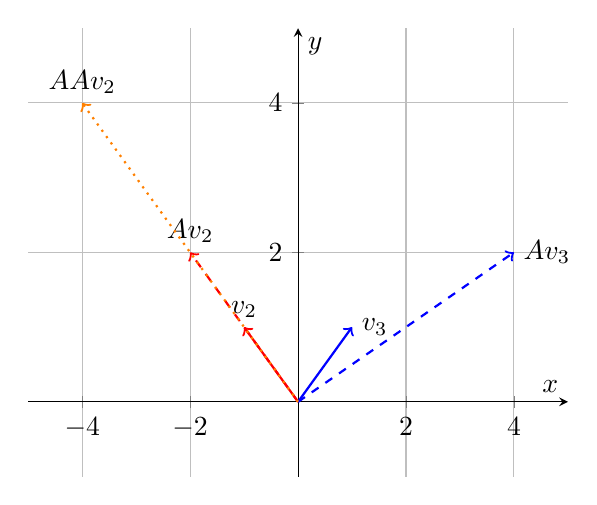
\begin{tikzpicture}
    \begin{axis}[
        axis lines=middle, 
        grid=major, 
        xlabel={$x$}, 
        ylabel={$y$}, 
        ymin=-1, ymax=5,
        xmin=-5, xmax=5
    ]
        % Define original vectors
        \addplot[->, thick, red] coordinates {(0,0) (-1, 1)};
        \node[above] at (axis cs:-1,1) {$v_2$};
        
        \addplot[->, thick, blue] coordinates {(0,0) (1,1)};
        \node[right] at (axis cs:1,1) {$v_3$};

        % Define transformed vectors
        \addplot[->, thick, red, dashed] coordinates {(0,0) (-2,2)};
        \node[above] at (axis cs:-2,2) {$A v_2$};
        
        \addplot[->, thick, blue, dashed] coordinates {(0,0) (4,2)};
        \node[right] at (axis cs:4,2) {$A v_3$};

        \addplot[->, thick, orange, dotted] coordinates {(0,0) (-4,4)};
        \node[above] at (axis cs:-4,4) {$A A v_2$};
    \end{axis}
\end{tikzpicture}
\end{center}
Et c'est pas uniquement le cas du vecteur $\begin{pmatrix} -1 \\ 1 \end{pmatrix} $, en prennant n'importe quel vecteur engendré pas $v = \begin{pmatrix} -1 \\ 1 \end{pmatrix} $, on obtiendra $Av = 2v$.
Tels vecteurs $v$ et les scalaire (ici: 2) sont appelés vecteurs propres et valeurs propres respectivement. Alors, on a la définition formelle:
\begin{definition}
    Soit $f$ un endomorphisme dans  $E$ et un vecteur  $v \in E$ est dit \textbf{vecteur propre} de $f$ si:
     \begin{enumerate}
        \item $v \neq 0$
        \item Il existe un réél $\lambda$ tel que  $f(v) = \lambda v$
    \end{enumerate}
    Le scalaire $\lambda \in \R$ est dit \textbf{valeur propre} correspondante à $v$.
\end{definition}
\begin{intuition}
   Les vecteurs propres sont les vecteurs qui sous l'action de $f$ ne changent pas de diréctions, justement la longueure (même pas toujours). Cela simplifie le calcul de tel vecteurs. Pouvez-vous calculer  $A^3v_3$? Pas très facile, alors le vecteur  $A^3v_2$? 
   \[
    Av_2 = 2v_2 \implies A^2v_2 = 2\cdot 2v_2 = 4v_2 \implies A^3v_2 = 2 \cdot 4v_2 = 8v_2 = \begin{pmatrix} -8 \\ 8 \end{pmatrix} 
   \] 
   C'est cool, n'est-ce pas?
\end{intuition}
Par contre, ce n'est pas la seule utilité des vecteurs propres et on va revenir ici pour en discuter, mais d'abord, comment trouver tels vecteurs?

\section{Recherche des valeurs propres}
On cherche des vecteurs qui sous l'action de l'endomorphisme $f$ sont mis à l'échelle par un facteur de  $\lambda \in \R$, alors on est sensé de résoudre cette équation:
\begin{align*}
    && f(v) &= \lambda v\\
    \iff&& Av &= \lambda v \quad \text{ en notation matricielle}\\
    \iff&& Av &= \lambda (Iv) \quad \text{ où } I \text{ est une matrice identité}\\
    \iff&& Av - \lambda Iv &= 0\\
    \iff&& (A - \lambda I)v &= 0
\end{align*}
Donc, on doit étudier l'application $(A - \lambda I)$ et la connecter à la notion des détérminants. Rappelle: si le détérminant d'une matrice n'est pas nul, cette matrice (i.e endomorphisme) est injective. Dans notre cas, si  $\det(A - \lambda I)$ était nul, le seul vecteur  $v$ qui donnerait  $(A - \lambda I)v = 0$ était le vecteur nul  $v = 0$ car  $(A - \lambda I)$ est linéaire et (comme on a suppoé) injective. 
\par
Par contre, d'après la définition, les vecteurs propres ne sont pas nul, alors le cas injectif ne convient pas, donc pour avoir des vecteurs propres l'application $(A - \lambda I)$ doit ne pas être injectif ce qui équivaut à dire que  $\det(A - \lambda I) = 0$. Alors, on est sensé de calculer le détérminant suivant:
\[
\det(A - \lambda I) = \det \left(\begin{bmatrix} 
    a_{1,1} & a_{1, 2} & \ldots & a_{1, n}\\
    a_{2,1} & a_{2, 2} & \ldots & a_{2, n}\\
    \ldots & \ldots & \ldots & \ldots\\
    a_{n,1} & a_{n,2} & \ldots & a_{n,n}
    \end{bmatrix}  - 
    \begin{bmatrix} 
        \lambda & 0 & \ldots & 0 \\
        0 & \lambda & \ldots & 0 \\
        \ldots & \ldots & \ldots & \ldots\\
        0 & 0 & \ldots & \lambda
    \end{bmatrix}\right) = 
    \begin{vmatrix} 
    a_{1,1} - \lambda & a_{1, 2} & \ldots & a_{1, n}\\
    a_{2,1} & a_{2, 2} - \lambda & \ldots & a_{2, n}\\
    \ldots & \ldots & \ldots & \ldots\\
    a_{n,1} & a_{n,2} & \ldots & a_{n,n} - \lambda
    \end{vmatrix}
\] 
En développant ce détérminant on obtient une équiation du type:
\[
    (-1)^n\lambda^n + a_{n-1}\lambda^{n-1} + \ldots + a_1\lambda + a_0 = 0
\] 
dont les racines sont les valeurs propres de $f$ (rappelle: valeur propre est un facteur $\lambda$).
Ne vous concentrez pas trop sur cette équation pour l'instant, on va y revenir.
\begin{prop}
   Soit $f$ un endomorphisme dans un espace vectoriel  $E$ de dimension finie  $n$ et $A$ la matrice représentative de  $f$ dans une base de  $E$. Les valeurs propres de  $f$ sont les racine du polynôme:
   \[
   P_f(\lambda) = \det(A - \lambda I)
   \] 
\end{prop}
Pour clarifier:
\begin{eg}
   Soit $f$ un endomorphisme dans  $\R^2$ dont la matrice représentative dans la base canonique est:
   \[
       \begin{bmatrix} 3 & 1\\ 0 & 2 \end{bmatrix} 
   \] 
   Calculons ses valeurs propres:
   \begin{align*}
       && \begin{bmatrix} 3 & 1\\ 0 & 2 \end{bmatrix} v &= \lambda v \\
       \iff && \begin{bmatrix} 3 & 1\\ 0 & 2 \end{bmatrix} v - \lambda I v &= 0\\
       \iff && \left(\begin{bmatrix} 3 & 1\\ 0 & 2 \end{bmatrix}  - \lambda I\right)v  &= 0\\
       \implies && \det \left( \begin{bmatrix} 3 & 1\\ 0 & 2 \end{bmatrix}  - \lambda I \right) &= 0\\
       \implies && \det \left( \begin{bmatrix} 3 & 1\\ 0 & 2 \end{bmatrix}  - \lambda \begin{bmatrix} \lambda & 0\\ 0 & \lambda \end{bmatrix}  \right) &= 0\\
       \implies && \det \left( \begin{bmatrix} 3 - \lambda & 1\\ 0 & 2 - \lambda \end{bmatrix}\right) &= 0\\
                && &= (3-\lambda)(2 - \lambda) = 0
   \end{align*}
   On voit bien, que les solutions sont: $\lambda_1 = 3$ et  $\lambda_2 = 2$
\end{eg}
On peut trouver des valeurs propres, néanmoins, on cherchait les \underline{vecteurs} propres. Et on est là:
\section{Recherche des vecteurs propres}
Supposons pour $q \in \N^{*}$ on a déjà trouvé $q$ valeurs propres d'une matrice $\{ \lambda_1, \ldots, \lambda_q \}$, pour trouver les vecteurs propres, il nous reste à trouver la base de:
\[
    \ker(A - \lambda_iI) \quad \forall i \in \{1, \ldots, q\}
\] 
ce qui équivaut à:
\[
\left( A - \lambda_i I \right)v = 0 \quad \forall i \in \{1, \ldots, q\}
\] 

\begin{eg}
   Encore la matrice  
   \[
       A = \begin{bmatrix} 3 & 1\\ 0 & 2 \end{bmatrix} 
   \] 
   dans la base canonique de $\R^2$. On a déjà trouvé ses vecteurs propres: $\lambda_1 = 3$ et $\lambda_2 = 2$. Alors, cherchons les vecteurs:
   \[
       \begin{bmatrix} 3 - \lambda_1 & 1 \\ 0 & 2 - \lambda_1 \end{bmatrix}\begin{bmatrix} x \\ y \end{bmatrix} = \begin{bmatrix} 3 - 3 & 1 \\ 0 & 2 - 3 \end{bmatrix}\begin{bmatrix} x \\ y \end{bmatrix} = \begin{bmatrix} 0 & 1 \\ 0 & -1 \end{bmatrix}\begin{bmatrix} x \\ y \end{bmatrix} = 0 
       \implies \begin{cases}
           y = 0\\
           -y = 0\\
           x \in \R
       \end{cases}
   \] 
   Donc $\ker(A - 3I) = \begin{pmatrix} x \\ 0 \end{pmatrix} =  \operatorname{Vect}(\begin{pmatrix} 1 \\ 0 \end{pmatrix} )$. Voilà, notre premier vecteur propre: $\begin{pmatrix} 1 \\ 0 \end{pmatrix} $. Pour le deuxième:
   \[
       \begin{bmatrix} 3 - \lambda_2 & 1 \\ 0 & 2 - \lambda_2 \end{bmatrix}\begin{bmatrix} x \\ y \end{bmatrix} = \begin{bmatrix} 3 - 2 & 1 \\ 0 & 2 - 2 \end{bmatrix}\begin{bmatrix} x \\ y \end{bmatrix} = \begin{bmatrix} 1 & 1 \\ 0 & 0 \end{bmatrix}\begin{bmatrix} x \\ y \end{bmatrix} = 0 
       \implies \begin{cases}
           x + y = 0
       \end{cases} \implies \begin{cases}
           x = -y
       \end{cases}
   \] 
   Donc $\ker(A - 2I) = \begin{pmatrix} -y \\ y \end{pmatrix} = y \begin{pmatrix} -1 \\ 1 \end{pmatrix} = \operatorname{Vect}(\begin{pmatrix} -1 \\ 1 \end{pmatrix} )  $ et voilà le deuxieme vecteur propre: $\begin{pmatrix} -1 \\ 1 \end{pmatrix} $ (c'était notre vecteur $v_2$ au début du chapitre).
\end{eg}

Enfin, la propriété utile:
\begin{prop}
    Soit $A \in \mathcal{M}_n(\R)$ avec ses vecteurs propres: $\{\lambda_1, \ldots, \lambda_n\}$, alors:
    \begin{align*}
        &\operatorname{Tr}(A) = \lambda_1 + \ldots + \lambda_n\\
        &\operatorname{det}(A) = \lambda_1 \cdot  \ldots \cdot  \lambda_n\\
    \end{align*}
\end{prop}

\section{Les endomorphismes diagonalisables}
Revenons sur l'utilité des vecteurs propres. Soit $f$ un endomorphisme de  $E$ dont la base est  $\{e_1, \ldots, e_n\}$ et $\operatorname{Mat}_{e_i}(f) = A$ et la matrice de  $f$ dans cette base. Reprennons l'exemple suivant:
 \begin{eg}
     On a: $A = \begin{bmatrix} 3 & 1\\ 0 & 2 \end{bmatrix} $ dans la base canonique $e_1 = \begin{bmatrix} 1 \\ 0 \end{bmatrix} $ et $e_2 = \begin{bmatrix} 0 \\ 1 \end{bmatrix} $. On rappelle qu'on a trouvé deux vecteurs propres:
     \[
     \begin{cases}
         v_1 = \begin{pmatrix} 1 \\ 0 \end{pmatrix} \\
         v_2 = \begin{pmatrix} -1 \\ 1 \end{pmatrix} 
     \end{cases}
     \] 
     On remarque que ces deux vecteurs sont libres et donc forment une base  de $\R^2$. Essayons de changer la base de $A$ dont on a deux façon:
      \begin{enumerate}
          \item On peut calculer les coordonnées de $f(v_1)$ et $f(v_2)$ dans la base $\{v_1, v_2\}$, on a:
              \begin{align*}
                  &f(v_1) = 3v_1 = 3 \cdot v_1 + 0 \cdot v_2\\
                  &f(v_2) = 2v_2 = 0 \cdot v_0 + 2 \cdot v_2
              \end{align*}
              Et alors $\operatorname{Mat}_{v_i}(f) = \|f(v_1), f(v_2)\|_{v_i} = \begin{bmatrix} 3 & 0 \\ 0 & 2 \end{bmatrix} $ 
          \item On peut calculer la matrice $P = P_{e_i \to v_i}$de passage d'une base $\{e_i\}$ vers la base  $\{v_i\}$ et en déduire la matrice de $f$ dans la nouvelle base. On a:
             \[
            \begin{cases}
                v_1 = \begin{pmatrix} 1 \\ 0 \end{pmatrix} = 1 \cdot e_1 + 0 \cdot e_2 = \begin{pmatrix} 1 \\ 0 \end{pmatrix}_{e_i} \\
                v_2 = \begin{pmatrix} -1 \\ 1 \end{pmatrix} = -1 \cdot e_1 + 1 \cdot e_2 = \begin{pmatrix} -1 \\ 1 \end{pmatrix}_{e_i} \\
            \end{cases}
            \] 
              donc $P = \begin{bmatrix} 1 & -1\\ 0 & 1 \end{bmatrix} $ et $P^{-1} = \begin{bmatrix} 1 & 1 \\ 0 & 1  \end{bmatrix}$ (vous pouvez vérifier le calcul). Et donc:
              \[
                  A' = P^{-1}AP = \begin{bmatrix} 1 & 1 \\ 0 & 1 \end{bmatrix} \begin{bmatrix} 3 & 1 \\ 0 & 2 \end{bmatrix} \begin{bmatrix} 1 & -1 \\ 0 & 1 \end{bmatrix} = \begin{bmatrix} 1 & 1 \\ 0 & 1 \end{bmatrix} \underbrace{\begin{bmatrix} 3 & -2 \\ 0 & 2 \end{bmatrix}}_{AP} = \begin{bmatrix} 3 & 0 \\ 0 & 2 \end{bmatrix} 
              \] 
     \end{enumerate}
     Et voilà, la magie, on a trouvé la matrice diagonale.
\end{eg}
Ensuite, généralisons ce qu'on a fait. 
\begin{definition}
    Soit $\lambda \in K$, on note:
    \[
        E_{\lambda} := \{v \in E \mid f(v) = \lambda v \}
    \] 
    $E_{\lambda}$ est un espace vectoriel de $E$ dit  \textbf{espace propre} correspondant à $\lambda$.
\end{definition}
\begin{remark}
   \begin{enumerate}
       \item Si $\lambda$ n'est pas valeur propre de $f$, donc  $E_\lambda = \{0\}$
       \item Si  $\lambda$ est valeur propre, alors:
            \[
                E_\lambda = \{ \text{ vecteurs propres associés à } \lambda \} \cup \{0\} \text{ et } \dim E_\lambda \ge 1
           \] 
   \end{enumerate} 
\end{remark}


% \begin{tikzpicture}
%     \begin{axis}[
%         axis lines=middle, 
%         grid=major, 
%         xlabel={$x$}, 
%         ylabel={$y$}, 
%         title={Eigenvector Transformation},
%         ymin=-2, ymax=5,
%         xmin=-3, xmax=5
%     ]
%         % Define original vectors
%         \addplot[->, thick, red] coordinates {(0,0) (1,0)};
%         \node[right] at (axis cs:1,0) {$v_1$};
%
%         \addplot[->, thick, red] coordinates {(0,0) (-1, 1)};
%         \node[above] at (axis cs:-1,1) {$v_2$};
%
%         \addplot[->, thick, blue] coordinates {(0,0) (1,1)};
%         \node[right] at (axis cs:1,1) {$v_3$};
%
%         \addplot[->, thick, blue] coordinates {(0,0) (-1,2)};
%         \node[left] at (axis cs:-1,2) {$v_4$};
%
%         % Define transformed vectors
%         \addplot[->, thick, red, dashed] coordinates {(0,0) (3,0)};
%         \node[right] at (axis cs:3,0) {$A v_1$};
%
%         \addplot[->, thick, red, dashed] coordinates {(0,0) (-2,2)};
%         \node[above] at (axis cs:-2,2) {$A v_2$};
%
%         \addplot[->, thick, blue, dashed] coordinates {(0,0) (4,2)};
%         \node[right] at (axis cs:4,2) {$A v_3$};
%
%         \addplot[->, thick, blue, dashed] coordinates {(0,0) (-1,4)};
%         \node[left] at (axis cs:-1,4) {$A v_4$};
%     \end{axis}
% \end{tikzpicture}
